\documentclass[10pt]{article}
\usepackage{amsmath, amssymb, graphics,color}
\usepackage{xcolor}

\begin{document}

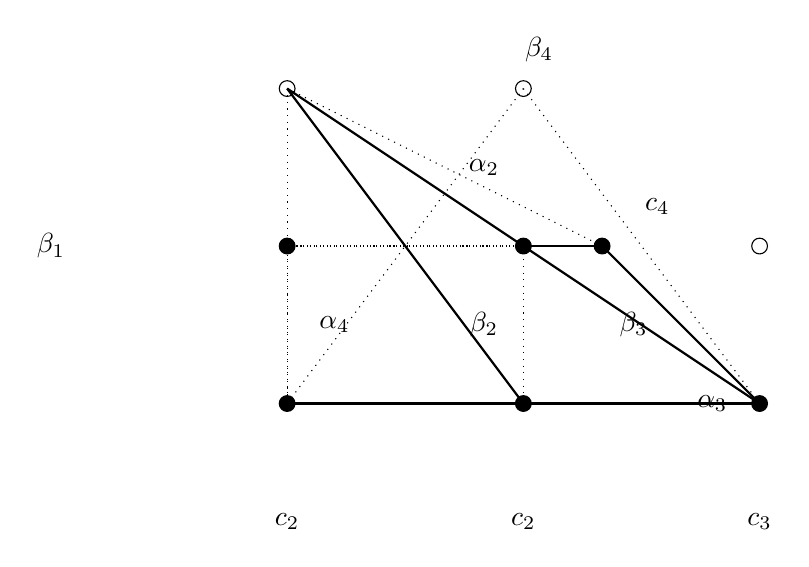
\begin{tikzpicture}
% Vertices
\draw [fill=black] (2,1) circle [radius=0.1];
\draw [fill=black] (5,1) circle [radius=0.1];
\draw [fill=black] (8,1) circle [radius=0.1];
\draw [fill=black] (6,3) circle [radius=0.1];
\draw [fill=black] (2,3) circle [radius=0.1];
\draw [fill=black] (5,3) circle [radius=0.1];
\draw [fill=white] (8,3) circle [radius=0.1];
\draw [fill=white] (2,5) circle [radius=0.1];
\draw [fill=white] (5,5) circle [radius=0.1];

% Edges
\draw [thick] (2, 1) -- (5, 1);
\draw [thick] (5, 1) -- (8, 1);
\draw [thick] (6, 3) -- (8, 1);
\draw [thick] (5, 3) -- (8, 1);
\draw [thick] (5, 3) -- (6, 3);
\draw [thick] (2, 5) -- (5, 3);
\draw [thick] (2, 5) -- (5, 1);

\draw [dotted] (5,5) -- (8,1);
\draw [dotted] (5,5) -- (2,1);
\draw [dotted] (2,5) -- (2,1);
\draw [dotted] (2,5) -- (8,1);
\draw [dotted] (5,3) -- (5,1);
\draw [dotted] (6,3) -- (8,1);
\draw [dotted] (6,3) -- (5,3);
\draw [dotted] (5,3) -- (2,3);
\draw [dotted] (2,3) -- (2,1);
\draw [dotted] (2,3) -- (6,3);
\draw [dotted] (2,5) -- (6,3);

% Labels
\node at (2, -0.5) {$c_2$};
\node at (5, -0.5) {$c_2$};
\node at (8, -0.5) {$c_3$};
\node at (6.7, 3.5) {$c_4$};
\node at (5.2, 5.5) {$\beta_4$};
\node at (-1, 3) {$\beta_1$};
\node at (2.6, 2) {$\alpha_4$};
\node at (4.5, 4) {$\alpha_2$};
\node at (7.4, 1) {$\alpha_3$};
\node at (4.5, 2) {$\beta_2$};
\node at (6.4, 2) {$\beta_3$};

\end{tikzpicture}

Remaining vertices of the six hyperedges in which Breaker has not yet played in Case 1 of Theorem~\ref{TD(4,4)}. These hyperedges are $\{\alpha_3, \beta_2\}$, $\{c_2, \alpha_2, \beta_2\}$, $\{c_2, \alpha_4, \beta_1\}$, $\{c_3, \alpha_3, \beta_3\}$, $\{c_4, \alpha_2, \beta_3\}$, and $\{c_4, \alpha_4, \beta_4\}$.

\end{document}